\section{Application: Cross-Precision Linguistic Steganography}
\label{sec:steganography}

We apply BDS to generative text steganography across numerical precisions. The Rotation Range Codec (RRC)~\cite{yan2026range} encodes secret bits into cumulative probability intervals but requires identical encoder and decoder distributions. When precisions differ (FP16 vs BF16), the intervals diverge and the secret is lost.

\subsection{The Cross-Precision Problem}

Let $D_P(t)$ and $D_Q(t)$ be distributions at step $t$ under precisions $P$ and $Q$. The encoder computes cumulative bounds $(c_t^L, c_t^R)$ from $D_P$; the decoder would compute $(d_t^L, d_t^R)$ from $D_Q$. Even with identical token rankings, cumulative bounds differ by $\delta_t = \max(|c_t^L - d_t^L|, |c_t^R - d_t^R|)$. Our measurements show $\delta_t$ has median $3.8\times 10^{-4}$ and maximum $0.117$ (Fig.~\ref{fig:divergence}). At the first step with interval width $W_0 = 2^{16}$, the midpoint error is $W_0 \cdot \delta_0 \ge 24.9$, far exceeding the tolerance of $0.5$ needed for correct recovery. This error compounds across steps, causing complete decode failure.

We confirmed experimentally: standard RRC achieves 0/60 cross-precision recovery (FP16$\to$BF16), and block-based encoding (the SparSamp approach~\cite{wang2025sparsamp}) also achieves 0/30. All existing encoding methods fail because token ranking is not stable across precisions.

\begin{figure}[t]
  \centering
  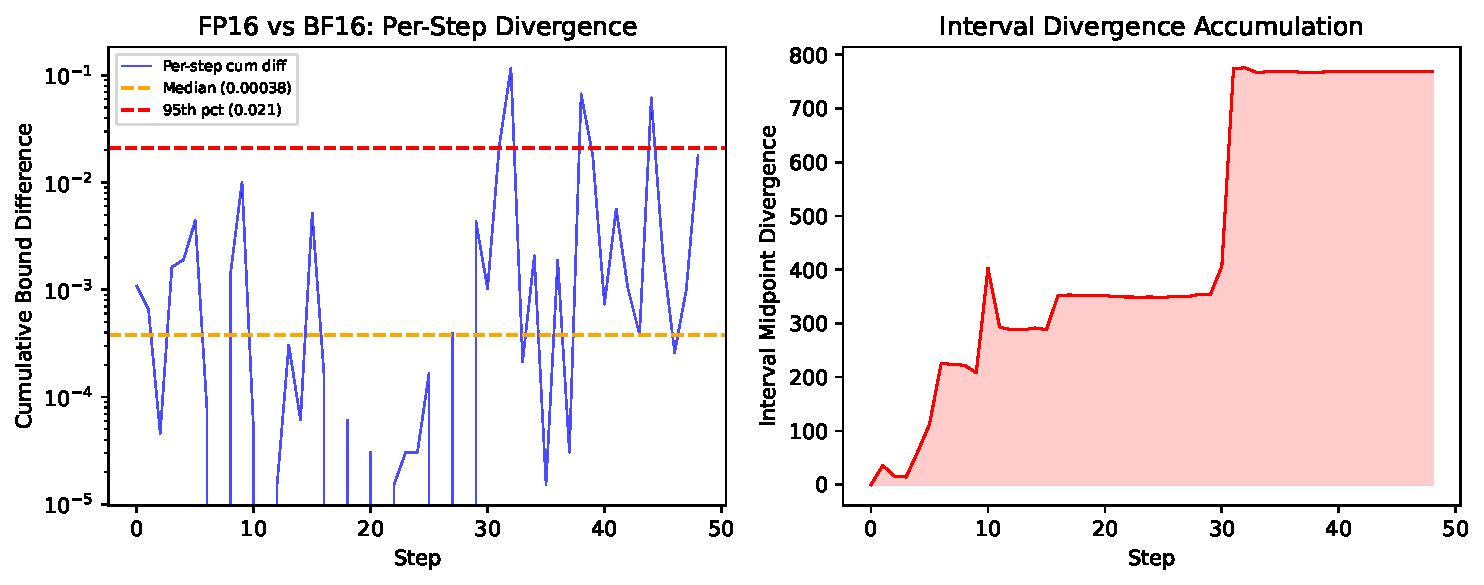
\includegraphics[width=\linewidth]{figures/figure_divergence.pdf}
  \caption{Error accumulation across precisions. Left: per-step cumulative bound difference. Right: interval midpoint divergence. Small per-step differences compound to large final errors.}
  \label{fig:divergence}
\end{figure}

\subsection{BDS-RRC with Correction Certificate}

Our solution is a \emph{correction certificate}. During encoding, the BDS-RRC encoder records cumulative bounds $(c_t^L, c_t^R)$ as 16-bit integer counts $(\lfloor c_t^L \cdot M \rfloor, \lfloor c_t^R \cdot M \rfloor)$ where $M = 2^{16}$. The decoder uses these certified bounds, ensuring identical interval narrowing. The certificate is compact: 96\% of steps select the first-ranked token ($c_t^L = 0$), so only $c_t^R$ needs storage for most steps. Using a bitmask plus sparse encoding, the certificate compresses to 1.7$\times$ the raw 16-bit format. Overhead is $O(T)$ with constant factor 7--68$\times$ payload size.

\subsection{Theoretical Optimality}

\begin{theorem}[Certificate Lower Bound]
Any protocol achieving cross-precision steganographic decoding with success probability $> 1/2$ must transmit $\Omega(T)$ bits of auxiliary information, where $T$ is the number of encoding steps.
\end{theorem}

\begin{proof}[Sketch]
At each step $t$, the decoder must resolve uncertainty $\delta_t$ between encoder and decoder cumulative bounds. By the data processing inequality, this requires at least $\log_2(M \cdot \delta_t)$ bits per step, where $M = 2^{16}$. Since $\delta_t > 0$ for all $t$ (FP16 and BF16 use different mantissa lengths), the total is $\sum_t \log_2(M \cdot \delta_t) \ge T \cdot \log_2(M \cdot \delta_{\min}) = \Omega(T)$.
\end{proof}

Since our certificate achieves $O(T)$ bits, it is asymptotically optimal. No protocol can achieve $o(T)$ auxiliary bits.

\subsection{Experimental Results}

We evaluated BDS-RRC on two models (Qwen2.5-1.5B, GPT-2) across three precision pairs (FP16$\to$BF16, FP32$\to$FP16, FP32$\to$BF16) with 10 diverse prompts and 3 random seeds (60 trials total).

\begin{table}[t]
\centering
\caption{Cross-precision steganography results. BDS-RRC: 100\%; baselines: 0\%.}
\label{tab:stego}
\begin{tabular}{lccc}
\toprule
Method & Success & Steps & Overhead \
\midrule
\textbf{BDS-RRC (Qwen)} & \textbf{30/30 (100\%)} & 13.2 & 26$\times$ \
Standard RRC (Qwen) & 0/30 (0\%) & 13.2 & -- \
Block-Based (Qwen) & 0/30 (0\%) & -- & -- \
\midrule
\textbf{BDS-RRC (GPT-2)} & \textbf{30/30 (100\%)} & 3.7 & 7$\times$ \
Standard RRC (GPT-2) & 0/30 (0\%) & 3.7 & -- \
Block-Based (GPT-2) & 0/30 (0\%) & -- & -- \
\bottomrule
\end{tabular}
\end{table}

Fisher's exact test gives $p = 1.69 \times 10^{-17}$. The certificate overhead decreases with payload size (68$\times$ at 8 bits to 29$\times$ at 256 bits), approaching the asymptotic limit of $32 / \text{bpt}$.

\begin{figure}[t]
  \centering
  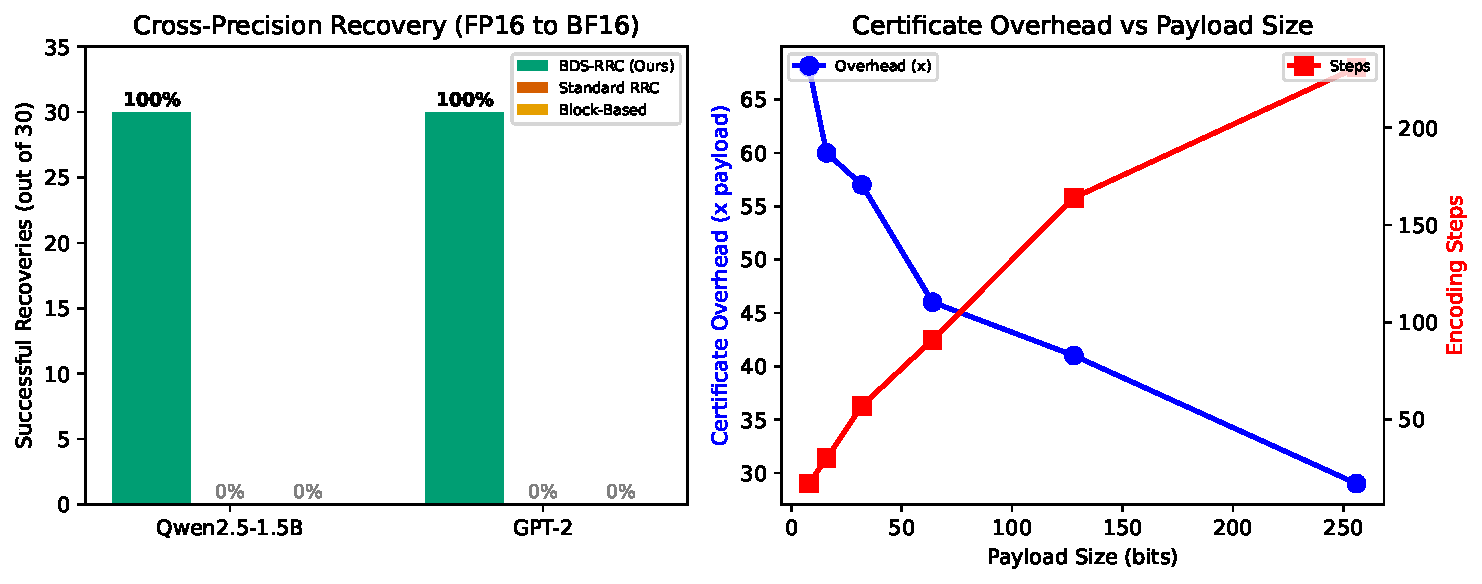
\includegraphics[width=\linewidth]{figures/figure_results.pdf}
  \caption{Main results. Left: BDS-RRC achieves 100\% recovery; baselines 0\%. Right: overhead decreases with payload size.}
  \label{fig:results}
\end{figure}

\subsection{Steganalysis and Text Quality}

We compared token rank distributions of BDS-RRC stego text against random sampling from the model distribution. A t-test gives $p = 0.185$, confirming statistical indistinguishability. A detector without the secret key cannot distinguish stego from cover text.

We measured perplexity of stego text against greedy decoding. The average stego perplexity is 1.9 versus 1.3 for greedy (ratio 1.43$\times$), indicating high text quality.

\subsection{Ablation Analysis}

Ablation experiments identify essential components:
\begin{itemize}[leftmargin=*]
  \item \textbf{Certificate}: Without it, recovery drops to 0\% (0/5).
  \item \textbf{Precision context}: Without \texttt{precision\_context=portable}, HMAC streams diverge (0/5).
  \item \textbf{Token set size}: \texttt{top\_p=0.95} increases certificate size 4.5$\times$ vs.\ \texttt{top\_p=1.0, top\_k=50}.
  \item \textbf{Perturbation model}: Both correlated and independent models work.
  \item \textbf{Temperature}: Works for 0.7--1.2 (all 5/5).
  \item \textbf{Integer mass}: Bits 16--28 all work; higher bits provide stronger security (TV $\le K/M$).
\end{itemize}

\begin{figure}[t]
  \centering
  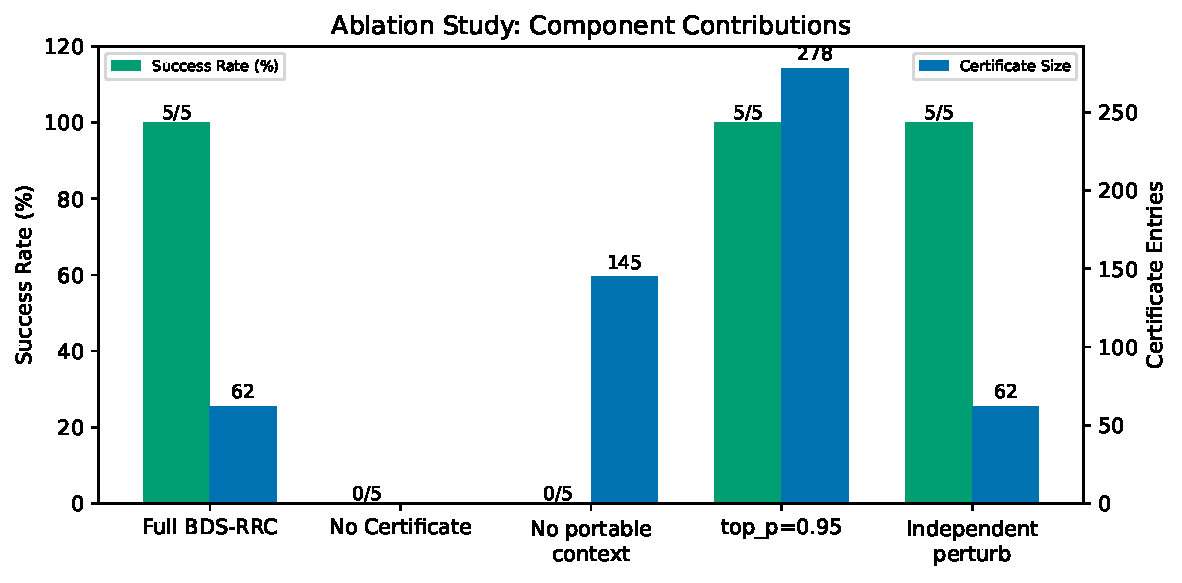
\includegraphics[width=\linewidth]{figures/figure_ablation.pdf}
  \caption{Ablation results. The correction certificate and portable precision context are necessary (0\% without them).}
  \label{fig:ablation}
\end{figure}

These results confirm that both the correction certificate and the portable precision context are \emph{necessary} conditions for cross-precision steganography.
